\documentclass[a4paper,11pt]{scrartcl}
\usepackage[ngerman]{babel}
\usepackage[utf8]{inputenc}

\usepackage{amssymb}
\usepackage{amsmath}
\usepackage{commath}
\usepackage[retainorgcmds]{IEEEtrantools}

\usepackage[ngerman]{cleveref}
\usepackage{graphicx}
\usepackage{enumitem}

\newcommand*{\eps}{\varepsilon}
\newcommand*{\sm}{\sum_{i=0}^\infty}
\newcommand*{\Ld}{\mathcal{O}}
\newcommand*{\pyi}[1]{\frac{\partial{#1}}{\partial y_i}}
\newcommand*{\pxj}[1]{\frac{\partial{#1}}{\partial x_j}}
\newcommand*{\Dx}{\Delta{}x}
\newcommand*{\yt}{\tilde{y}}
\newcommand*{\dy}{\dif{}y}

\setlist[enumerate,2]{label=\textbf{\alph*)}}


\begin{document}
\begin{enumerate}[label*=\textbf{9.\arabic*.}]

% ==================== 9.1 ====================
\item
  \begin{enumerate}
  \item
    DGL als System:
    \[\begin{pmatrix}y'\\v'\end{pmatrix}=
      \begin{pmatrix}v\\-\eps v^3 - y\end{pmatrix}
    \]
    Linearisiert ist der 0 punkt ein Zentrum.
    Der nichtlineare Anteil hilft zusäzlich die Lösung beschränkt zu halten.
    Sieht man in der Skizze vom Phasenportrait in \cref{fig:phaseportrait_9.1a}.

    \begin{figure}
    \centering
    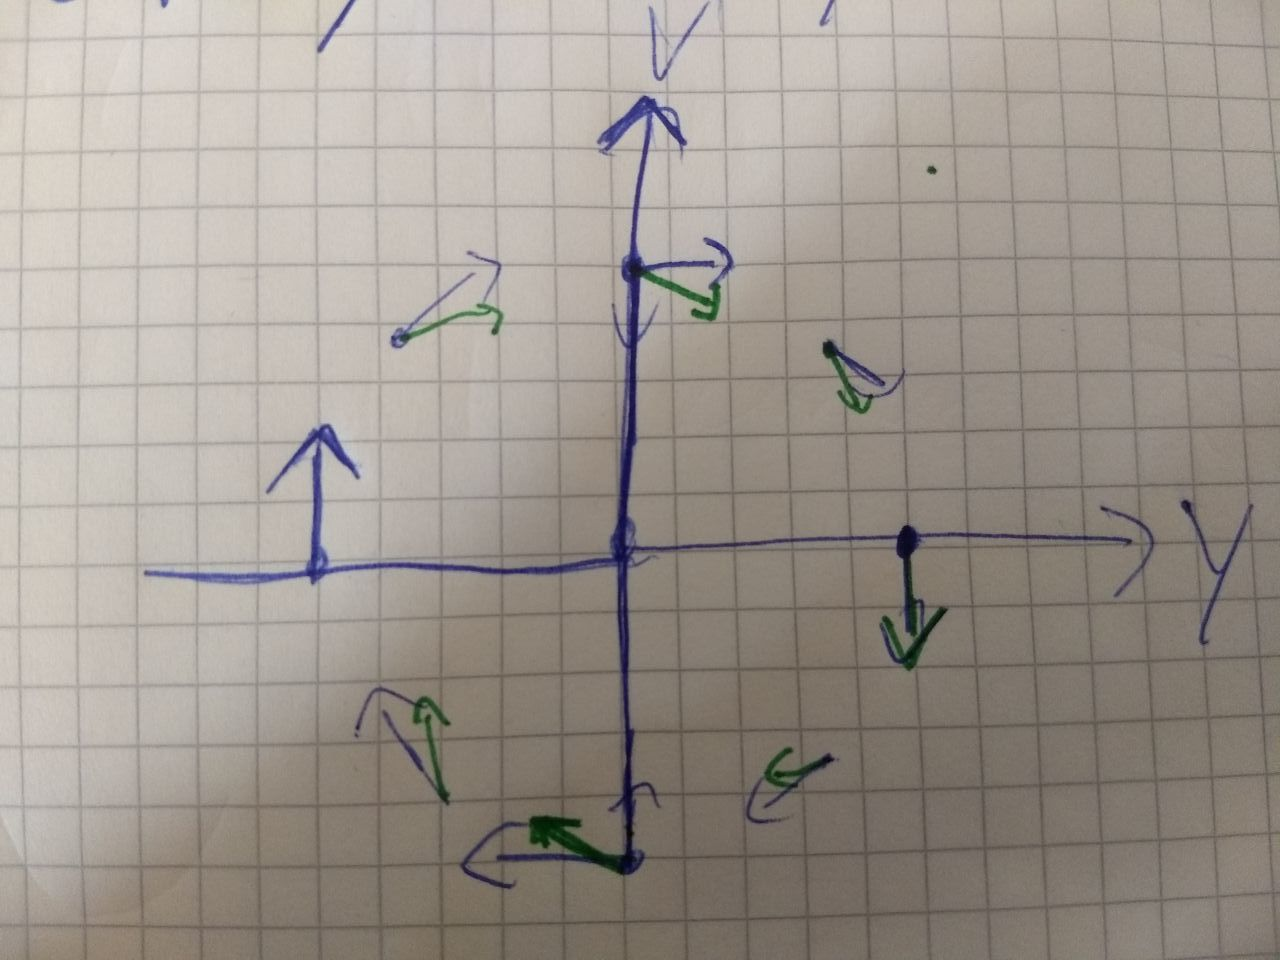
\includegraphics[width=.5\linewidth]{1a.jpg}
    \captionof{figure}{Skizze des Phasenportraits von 9.1a), blau: linearisiert, grün: nichtlinear}
    \label{fig:phaseportrait_9.1a}
    \end{figure}

  \item
    Mehrskalenansatz:
    \[ y = \sm \eps^i y_i(t, T), \quad \text{mit } T = \eps t \]
    \[ \Rightarrow y' = \sm \eps^i \partial_{1} y_i + \eps^{i+1} \partial_2 y_i\]
    \[ \Rightarrow y'' = \sm \eps^i \partial_{11} y_i + \eps^{i+1} \partial_{12}
      y_i + \eps^{i+1} \partial_{21} y_i + \eps^{i+2} \partial_{22} y_i\]

    Die DGL für den $\eps^0$ Term ist:
    \[ \partial_{11} y_0 + y_0 = 0\]
    Wie in der Vorlesung schreiben wir die allgemeine Lösung dafür als:
    \[ y_0 = r(T) \cos(t + \varphi(T))\]
    Die DGL für den $\eps^1$ Term ist:
    \[\partial_{11} y_1 + y_1 = - (\partial_1 y_0)^3 -2 \partial_{12} y_0\]
    \[\partial_1 y_0 = -r(T) \sin(t+\varphi(T)), \quad (\partial_1 y_0)^3 =
      -r^3(T) \frac{3 \sin(t + \varphi(T)) - \sin(3 (t + \varphi(T))}{4}\]
    \[\partial_{12} y_0 = -r'(T) \sin(t+\varphi(T)) - r(T) \cos(t + \varphi(T)) \varphi'(T) \]

    Daher ist die rechte Seite der $\eps^1$-Gleichung:
    \[\left(2r'(T) + \frac{3}{4} r^3(T)\right) \sin(t + \varphi(T)) + 2 r(T) \varphi'(T) \cos(t
     + \varphi(T)) - \frac{1}{4} r^3(T) \sin(3(t + \varphi(T))) \]

   Damit $y_1$ kein Wachstum in $t$ hat setzen wir die Terme vor den Lösungen der
   homogenen Gleichung auf 0.
   ($\sin(t), \cos(t)$ würden die homogene Gleichung lösen; $\sin(3t)$ nicht).
   \[ 2r'(T) + \frac{3}{4}r^3(T) = 0, \quad 2r(T)\varphi'(T) = 0\]
   Die erste Gleichung kann mittels Variablenseparation gelöst werden und die
   \[ r = \frac{1}{\sqrt{\frac{6}{8}T + c_1}}\]
   Aus der zweiten Gleichungt folgt $\varphi'(T) = 0 \Rightarrow \varphi(T) \equiv c_2$.

   Also
   \[y_0(t) = \frac{1}{\sqrt{\frac{6}{8}\eps t + c_1}} \cos(t + c_2)\]

   Die Konstanten können aus den Anfangsbedingungen ermittelt werden:
   \[a = y_0(0) = \frac{1}{\sqrt{c_1}} \cos(c_2) \Rightarrow
     (c_1)^{-\frac{1}{2}} = \frac{a}{\cos(c_2)}\]
   \[y'_0(t) = -\frac{3}{8}\eps \left(\frac{6}{8}\eps t +
       c_1\right)^{-\frac{3}{2}} \cos(t+c_2)- \left(\frac{6}{8}\eps t +
       c_1\right)^{-\frac{1}{2}} \sin(t + c_2)\]
   \[0 = y'_0(0) = -\frac{3}{8}\eps \left(c_1\right)^{-\frac{3}{2}} \cos(c_2)
     - \left(c_1\right)^{-\frac{1}{2}} \sin(c_2)
   = -\frac{3}{8} \eps \frac{a^3}{\cos^3(c_2)} \cos(c_2) - \frac{a\sin(c_2)}{\cos(c_2)}\]
 \[-\frac{3}{8} \eps a^2 = \sin(c_2)\cos(c_2) = \frac{1}{2}\sin(2c_2)\]
 \[c_2 = \frac{1}{2}\arcsin\left(\frac{-3}{8}\eps a^2\right)\]

\end{enumerate}


% ==================== 9.2 ====================
\item \begin{enumerate}
  \item
    Für die Energie multipliziert man die Gleichung mit $y'$ und integriert:
    \[\frac{(y')^2}{2} + \frac{y^2}{2} + \eps \frac{y^4}{4} = E\]

    System:
    \[\begin{pmatrix}y'\\v'\end{pmatrix}=
      \begin{pmatrix}v\\-\eps y^3 - y\end{pmatrix}
    \]

    Das Phasenportrait sieht ähnlich aus wie das Phasenportrait in
    \textbf{9.1a)}. Nur der nichtlineare Anteil wird durch $y$ verstärkt anstatt
    durch $v$.

    Auf jedem Orbit ist die Energie konstant, also auch im dem Punkt wo $y(t) =
    a \text{ und } y'(t) = 0$
    \[\Rightarrow E = \frac{a^2}{2}+\eps \frac{a^4}{4}\]
    \[\Rightarrow y'(t) = \sqrt{-y^2 - \eps \frac{y^4}{2} + a^2 + \eps \frac{a^4}{2}}\]
    \[\Rightarrow t'(y) = \frac{1}{\sqrt{-y^2 - \eps \frac{y^4}{2} + a^2 + \eps \frac{a^4}{2}}}\]

    Integral der Zeitableitung entlang eines Orbits ergibt die Periodendauer und
    $t'$ ist gerade ist gerade:
    \[T(\eps, a) = \int_a^0 t'(y) \dy + \int_0^{-a} t'(y) \dy + \int_{-a}^0
      t'(y) \dy + \int_0^a t'(y) \dy = 4 \int_0^a t'(y) \dy\]

    Als nächstes kommt die Taylor-Entwicklung von $T(\eps, a)$ in $\eps$ um 0:
    \[ \partial_\eps t'(y) = -\frac{1}{2} \left(-y^2 -\eps
          \frac{y^4}{2} + a^2 + \eps \frac{a^4}{2}\right)^{-\frac{3}{2}} \left(
          -\frac{y^4}{2} + \frac{a^4}{2} \right) \]
    \[ \partial_{\eps\eps} t'(y) = \frac{3}{4} \left(-y^2 -\eps
          \frac{y^4}{2} + a^2 + \eps \frac{a^4}{2}\right)^{-\frac{5}{2}} \left(
          -\frac{y^4}{2} + \frac{a^4}{2} \right)^2 \]

      \begin{IEEEeqnarray*}{rCl}
    T(\eps, a) &=& 4 \int_0^a \frac{1}{\sqrt{a^2 - y^2}} + \eps \frac{1}{2}
      \left( a^2 - y^2 \right)^{-\frac{3}{2}}\left( \frac{y^4}{2} -
        \frac{a^4}{2}\right) + \Ld(\eps^2) \dy \\
      &=& 4 \int_0^a \frac{1}{\sqrt{a^2 - y^2}}
      + \eps \frac{1}{4} \left(a^2 - y^2 \right)^{-\frac{3}{2}}(y^2 + a^2)(y^2-a^2)
      + \Ld(\eps^2) \dy \\
      &=& 4 \int_0^a \frac{1}{\sqrt{a^2 - y^2}}
      + \eps \frac{-1}{4} \sqrt{\frac{(a^2+y^2)^2}{a^2-y^2}} + \Ld(\eps^2) \\
      &=& 2 \pi - \eps \frac{3 \pi a^2}{4} + \Ld(\eps^2)
      \end{IEEEeqnarray*}
    
  \item
    Einsetzen der Reihenentwicklung von $\sin$ führt zu:
    \[ y'' + y - \frac{1}{6} y^3 = 0\]
    Das ist genau die Gleichung von \textbf{a)} mit $\eps = -\frac{1}{6}$.

    \[\Rightarrow T(a) = 2\pi + \frac{1}{8} \pi a^2 + \Ld(\eps^3)\]
    Und mit Taylor für $\frac{1}{x}$ erhält man:
    \[\omega = 2\pi f = \frac{2\pi}{T} \approx 1 - \frac{1}{16} a^2 \]

    
\end{enumerate}


% ==================== 9.3 ====================
\item
  \[\yt(\tau) = \yt\left(\frac{t}{\omega}\right)= y(t)\]
  \[\frac{1}{\omega^2} \yt'' = y''\]
  In die DGL einsetzen und mit $\omega^2$ multiplizieren.
  \[\yt'' + \omega^2 \yt + \eps \yt^3 = 0\]
  Jetzt führen wir die Entwicklungen durch wie in der Aufgabenstellung gegeben.
  $1$ als erster Term für die Entwicklung von Omega macht Sinn, da die Gleichung
  für $\eps=0$ eine Schwingung mit Kreisfrequenz $\omega=1$ ist.
  \[y''_0 + \eps y''_1 + (1 + 2 \eps \omega_1)(y_0 + \eps y_1) + \eps 
(1 + 2 \eps \omega_1) y^3_0 + \Ld(\eps^2)= 0\]

  \[\eps^0: y''_0 + y_0 = 0\]
  \[\eps^1: y''_1 + y_1 + 2 \omega_1 y_0 + y_0^3 = 0\]

  Aus der $\eps^0$ Gleichung folgt mit den Anfangswerten:
  \[y_0 = a \cos(t)\]
  Aus der $\eps^1$ Gleichung folgt mit der Identität $\cos^3(\theta) = \frac{3
    \cos(\theta) + \cos(3 \theta)}{4}$:
  \[y_1'' + y_1 = -2 \omega_1 a \cos(t) - a^3 \frac{3 \cos(t) + \cos(3t)}{4}\]
  Die Rezonanzterme werden unterdrückt so wie in \textbf{9.1a)} mit der gleichen
  Begründung.
  \[-2\omega_1 a - \frac{3}{4} a^3 = 0\]
  \[\Rightarrow \omega_1 = -\frac{3}{8} a^2\]


% ==================== 9.4 ====================
\item
  \[ \yt'' + \eps(\yt^2 - 1) \omega \yt' + \yt = 0\]
  \[ (y''_0 + \eps y''_1 + \eps^2 y''_2) + \eps (y^2_0 + 2 \eps y_0 y_1 - 1) (1
    + \eps \omega_1) (y'_0 + \eps y'_1) + (1 + 2 \eps \omega_1 + \eps^2 \omega^2_1
    + 2 \eps^2 \omega_2)
    (y_0 + \eps y_1 + \eps^2 y_2) + \Ld(\eps^3)\]
  \[ \eps^0: y''_0 + y_0 = 0\]
  \[ \eps^1: y''_1 + (y^2_0-1) y'_0 + y_1 + 2 \omega_1 y_0 = 0 \]
  \[ \eps^2: y''_2 + (y_0^2-1) y'_1 + y'_0 (y_0^2 \omega_1 - \omega_1 + 2 y_0 y_1)  + y_2 + 2 \omega_1 y_1 + \omega^2_1 y_0 + 2\omega_2 y_0 = 0\]

  Aus $\eps^0$ folgt:
  $y_0 = a \cos(t) + b \sin(t)$.

  Die Inhomogenität für $\eps^1$ ist:

  \[(a^2 \cos(t)^2  + 2ab \sin(t) \cos(t) + b^2 \sin^2 (t)- 1) (a \sin(t) - b
    \cos(t)) - \omega_1 (a \cos(t) + b \sin(t)) \]
  %   \[= \left(a^2 \frac{1
  %       +\cos(2t)}{2}-1\right)a \sin(t) - \omega_1 a \cos(t)\]
  % \[=\frac{a^3}{2} \sin(t) + \frac{a^3}{4} (\sin(3t) + \sin(t)) - \omega_1 a
  %   \cos(t) - a \sin(t)   \]


\[2\sin \theta \cos \varphi =\sin(\theta +\varphi )+\sin(\theta -\varphi )\]

% ==================== 9.5 ====================
\item \begin{enumerate}
  \item
    In jedem Punkt ist $\nabla \varphi(x)$ eine orthogonale Matrix $Q(x)$,
    da $\nabla\varphi(x)^{-1} = (\nabla \varphi(x))^\top$.
    Außerdem gilt auch $C_{\varphi^{-1}} \equiv I$, da $\nabla \varphi^{-1} =
    (\nabla \varphi)^{-1}$.

    Taylor-Restglied:
    \[\varphi(x) = \varphi(y) + \int_0^1 \nabla\varphi ((1 - t) y + t x) \cdot (x - y) \dif{}t\]

    \[\norm{\varphi(x) - \varphi(y)}_2 \leq \max_{w\in B} \norm{\nabla\varphi(w)} \norm{x-y}_2\]
    und $\norm{\nabla\varphi} = 1$, weil $\nabla\phi$ in jedem Punkt eine
    orthogonale Matrix ist.
    Das gleiche Argument gilt für $\nabla\phi^{-1}$ und somit gilt die Aussage.

  \item
    Aus \textbf{a)} gilt $G(x, y) = 0$.

    Zuerst nach $y_i$ und dann nach $x_j$ differenzieren führt zur gesuchten Identität:
    \[G(x, y) = \sum_k (\varphi_k(x) - \varphi_k(y))^2 - (x_k - y_k)^2 = 0\]
    \[\pyi{}G(x,y) = -2 \sum_k (\varphi_k(x) - \varphi_k(y)) \pyi{\varphi_k(y)}
      + 2 (x_i - y_i) = 0\]
    \[\pxj{}\pyi{}G(x,y) = -2 \sum_k \pyi{\varphi_k(y)} \pxj{\varphi_k(x)}
      + 2 \delta_{ij} = 0\]

    Also $(\nabla\varphi(y))^\top \nabla\varphi(x) = I$ auch für verschiedene
    Punkte $y, x \in B$.

  \item
    Es folgt, dass in konvexen Umgebungen von $x \in \Omega$ gilt: $(\nabla
    \varphi(y))^\top = \nabla \varphi(x)^{-1}$ und damit $\nabla \varphi(x) =
    \nabla \varphi(y)$. $\nabla\varphi$ ist lokal eine konstante orthogonale
    Matrix $Q$. Damit $\varphi(x) = Q x + a$.

\end{enumerate}

\end{enumerate}
\end{document}